\documentclass[10pt]{article}
\usepackage[utf8]{inputenc}
\usepackage[T1]{fontenc}
\usepackage{amsmath}
\usepackage{amsfonts}
\usepackage{amssymb}
\usepackage[version=4]{mhchem}
\usepackage{stmaryrd}
\usepackage{bbold}
\usepackage{graphicx}
\usepackage[export]{adjustbox}
\usepackage{soul}  
\graphicspath{ {./images/} }

\title{MATH1002}

\author{Mingyuan Ba}
\date{\today}


\begin{document}
\maketitle

\section{Week 1}

\begin{enumerate}
\item  $\mathrm{A}$ vector $\mathbf{v}$ is a directed line segment that corresponds to a displacement from a point $A$ to a point $B$. The vector from $A$ to $B$ is denoted $\overrightarrow{A B}$, with $A$ the initial point or tail and $B$ the terminal point or head.

\item  The set of all points in $n$-dimensional space corresponds to the set of all vectors with tails at the origin $O$. To each point $A$, there corresponds the vector $\overrightarrow{O A}$, called the position vector of $A$.

\item  If $A$ is the point in the plane with coordinates $\left(a_{1}, a_{2}\right)$, then $\overrightarrow{O A}=\left[a_{1}, a_{2}\right]$. The entries $a_{1}$ and $a_{2}$ are the components of the vector $\overrightarrow{O A}$. We often use the column vector $\left[\begin{array}{l}a_{1} \\ a_{2}\end{array}\right]$ rather than the row vector $\left[a_{1}, a_{2}\right]$. Similarly if $A$ is the point in $n$-dimensional space with coordinates $\left(a_{1}, a_{2}, \ldots, a_{n}\right)$, \\\\
then the vector $\overrightarrow{O A}$ is $\left[a_{1}, a_{2}, \ldots, a_{n}\right]$ or $\left[\begin{array}{c}a_{1} \\ a_{2} \\ \vdots \\ a_{n}\end{array}\right]$, and this vector has $i$ th component $a_{i}$.

 \item  Two vectors are equal if and only if their corresponding components are equal. Geometrically, two vectors are equal if and only if they have the same length and the same direction, equivalently, we could translate one on to the other. A vector with its tail at the origin is in standard position.
\\\\
\textit{assignment2 - 2.3}

\item  The set of all vectors with $n$ components is denoted $\mathbb{R}^{n}$. This is the same as the set of all ordered $n$-tuples, written as row or column vectors.

\item  If $\mathbf{u}=\left[u_{1}, u_{2}\right]$ and $\mathbf{v}=\left[v_{1}, v_{2}\right]$ then their $\operatorname{sum} \mathbf{u}+\mathbf{v}$ is the vector $\mathbf{u}+\mathbf{v}=\left[u_{1}+v_{1}, u_{2}+v_{2}\right]$. Similarly in $\mathbb{R}^{n}$, if $\mathbf{u}=\left[u_{1}, u_{2}, \ldots, u_{n}\right]$ and $\mathbf{v}=\left[v_{1}, v_{2}, \ldots, v_{n}\right]$, then

$$
\mathbf{u}+\mathbf{v}=\left[u_{1}+v_{1}, u_{2}+v_{2}, \ldots, u_{n}+v_{n}\right]
$$

\item Head-to-Tail Rule for Vector Addition: Translate $\mathbf{v}$ so its tail is at the head of $\mathbf{u}$. Then $\mathbf{u}+\mathbf{v}$ is the vector from the tail of $\mathbf{u}$ to the head of $\mathbf{v}$.

\item Parallelogram Rule: If $\mathbf{u}$ and $\mathbf{v}$ are in standard position, then $\mathbf{u}+\mathbf{v}$ is the vector in standard position along the diagonal of the parallelogram determined by $\mathbf{u}$ and $\mathbf{v}$.

\item The zero vector in $\mathbb{R}^{n}$ is $\mathbf{0}=[0,0, \ldots, 0]=\overrightarrow{O O}$. This vector has length 0 and its direction is not defined. For all vectors $\mathbf{u}$ in $\mathbb{R}^{n}, \mathbf{u}+\mathbf{0}=\mathbf{u}$.

\item A scalar is a real number. Given a scalar $c$ and a vector $\mathbf{v}$, the scalar multiple c $\mathbf{v}$ is the vector obtained by multiplying each component of $\mathbf{v}$ by $c$. So if $\mathbf{v}=\left[v_{1}, v_{2}\right]$ then $c \mathbf{v}=\left[c v_{1}, c v_{2}\right]$. Similarly in $\mathbb{R}^{n}$, if $\mathbf{v}=\left[v_{1}, v_{2}, \ldots, v_{n}\right]$ then $c \mathbf{v}=\left[c v_{1}, c v_{2}, \ldots, c v_{n}\right]$. For all vectors $\mathbf{v}, 0 \mathbf{v}=\mathbf{0}$ and $1 \mathbf{v}=\mathbf{v}$, and for all scalars $c$ and $d, c(d \mathbf{v})=(c d) \mathbf{v}$. Geometrically, $c \mathbf{v}$ points in the same direction as $\mathbf{v}$ if $c>0$ and the opposite direction if $c<0$, and $c \mathbf{v}$ has length $|c|$ times the length of $\mathbf{v}$. Two vectors are scalar multiples of each other if and only if they are parallel.

\item The negative of a vector $\mathbf{v}$ is the vector $(-1) \mathbf{v}=-\mathbf{v}$. This has the same length as $\mathbf{v}$ but points in the opposite direction. For all vectors $\mathbf{v}, \mathbf{v}+(-\mathbf{v})=\mathbf{0}$. If $A$ and $B$ are points then $\overrightarrow{A B}=-\overrightarrow{B A}$.

\item We define vector subtraction by $\mathbf{u}-\mathbf{v}=\mathbf{u}+(-\mathbf{v})$.

\item If $P$ and $Q$ are points in $\mathbb{R}^{n}$ then $\overrightarrow{P Q}=\overrightarrow{O Q}-\overrightarrow{O P}$. (xiv) Commutative Law of Addition: For all vectors $\mathbf{u}$ and $\mathbf{v}$ in $\mathbb{R}^{n}, \mathbf{u}+\mathbf{v}=\mathbf{v}+\mathbf{u}$.

\item \hl{Associative Law of Addition} : For all vectors $\mathbf{u}, \mathbf{v}$ and $\mathbf{w}$ in $\mathbb{R}^{n},(\mathbf{u}+\mathbf{v})+\mathbf{w}=\mathbf{u}+(\mathbf{v}+\mathbf{w})$.

\item \hl{Distributive Laws}: For all scalars $c$ and $d$ and all vectors $\mathbf{u}$ and $\mathbf{v}$ in $\mathbb{R}^{n}, c(\mathbf{u}+\mathbf{v})=c \mathbf{u}+c \mathbf{v}$ and $(c+d) \mathbf{u}=c \mathbf{u}+d \mathbf{u}$

\end{enumerate}









\section{Week 2}
\begin{enumerate}

\item A vector $\mathbf{v}$ is a linear combination of vectors $\mathbf{v}_{1}, \mathbf{v}_{2}, \ldots, \mathbf{v}_{k}$ if there are scalars $c_{1}, c_{2}, \ldots, c_{k}$ such that

$$
\mathbf{v}=c_{1} \mathbf{v}_{1}+c_{2} \mathbf{v}_{2}+\cdots+c_{k} \mathbf{v}_{k}
$$

The scalars $c_{1}, c_{2}, \ldots, c_{k}$ are the coefficients of this linear combination.

\item The dot product of $\mathbf{u}=\left[u_{1}, u_{2}, \ldots, u_{n}\right]$ and $\mathbf{v}=\left[v_{1}, v_{2}, \ldots, v_{n}\right]$ is the scalar

$$
\mathbf{u} \cdot \mathbf{v}=u_{1} v_{1}+u_{2} v_{2}+\cdots+u_{n} v_{n}
$$


\newpage



\item \hl{Commutativity of dot product}: For all vectors $\mathbf{u}$ and $\mathbf{v}$ in $\mathbb{R}^{n}, \mathbf{u} \cdot \mathbf{v}=\mathbf{v} \cdot \mathbf{u}$.

\item \hl{Distributivity of dot product}: For all vectors $\mathbf{u}, \mathbf{v}$ and $\mathbf{w}$ in $\mathbb{R}^{n},(\mathbf{u}+\mathbf{v}) \cdot \mathbf{w}=\mathbf{u} \cdot \mathbf{w}+\mathbf{v} \cdot \mathbf{w}$.

\item For all scalars $c$ and all vectors $\mathbf{v}$ and $\mathbf{w}$ in $\mathbb{R}^{n},(c \mathbf{v}) \cdot \mathbf{w}=c(\mathbf{v} \cdot \mathbf{w})=\mathbf{v} \cdot(c \mathbf{w})$.

\item \hl{The length of a vector} $\mathbf{v}=\left[v_{1}, v_{2}, \ldots, v_{n}\right]$ in $\mathbb{R}^{n}$ is the scalar

$$
\|\mathbf{v}\|=\sqrt{\mathbf{v} \cdot \mathbf{v}}=\sqrt{v_{1}^{2}+v_{2}^{2}+\cdots+v_{n}^{2}}
$$

\textit{assignment1 -  1.3}
\item For all scalars $c$ and all vectors $\mathbf{v}$ in $\mathbb{R}^{n},\|c \mathbf{v}\|=|c|\|\mathbf{v}\|$.

\item \hl{A unit vector} is a vector of length one. Given any nonzero vector $\mathbf{v}$, the vector $\left(\frac{1}{\|\mathbf{v}\|}\right) \mathbf{v}$ is the unit vector in the same direction as $\mathbf{v}$, called the \hl{normalisation} of $\mathbf{v}$.

\textit{W3-tut - 2}

\item In $\mathbb{R}^{2}$ the unit vectors $\mathbf{e}_{1}=[1,0]$ and $\mathbf{e}_{2}=[0,1]$ lie along the positive $x$ - and $y$-axes, respectively. In $\mathbb{R}^{3}$ the unit vectors $\mathbf{e}_{1}=[1,0,0], \mathbf{e}_{2}=[0,1,0]$ and $\mathbf{e}_{3}=[0,0,1]$ lie along the positive $x-, y$ - and $z$-axes, respectively. \hl{In $\mathbb{R}^{n}$ we have the standard unit vectors $\mathbf{e}_{1}, \mathbf{e}_{2}, \ldots, \mathbf{e}_{n}$, where $\mathbf{e}_{i}$ has a 1 in its $i$ th component and 0 s elsewhere.}


\item \hl{Cauchy-Schwarz Inequality}: For all vectors $\mathbf{u}$ and $\mathbf{v}$ in $\mathbb{R}^{n},|\mathbf{u} \cdot \mathbf{v}| \leq\|\mathbf{u}\|\|\mathbf{v}\|$.

\item \hl{Triangle Inequality}: For all vectors $\mathbf{u}$ and $\mathbf{v}$ in $\mathbb{R}^{n},\|\mathbf{u}+\mathbf{v}\| \leq\|\mathbf{u}\|+\|\mathbf{v}\|$.

\item \hl{The distance between vectors} $\mathbf{u}$ and $\mathbf{v}$ in $\mathbb{R}^{n}$ is $d(\mathbf{u}, \mathbf{v})=\|\mathbf{u}-\mathbf{v}\|$.

\item The angle $\theta$ between nonzero vectors $\mathbf{u}$ and $\mathbf{v}$ in $\mathbb{R}^{n}$ is given by

$$
\cos \theta=\frac{\mathbf{u} \cdot \mathbf{v}}{\|\mathbf{u}\|\|\mathbf{v}\|}, \quad \text { with } 0 \leq \theta \leq \pi
$$

\item \hl{Two vectors $\mathbf{u}$ and $\mathbf{v}$ in $\mathbb{R}^{n}$ are orthogonal if $\mathbf{u} \cdot \mathbf{v}=0$, meaning that the angle between them is a right angle.}

\textit{assignment1 - 2.1}

\item \hl{If $\mathbf{u}$ and $\mathbf{v}$ are vectors in $\mathbb{R}^{n}$ and $\mathbf{u} \neq \mathbf{0}$, the projection of $\mathbf{v}$ onto $\mathbf{u}$ is the vector}

$$
\operatorname{proj}_{\mathbf{u}}(\mathbf{v})=\left(\frac{\mathbf{u} \cdot \mathbf{v}}{\|\mathbf{u}\|^{2}}\right) \mathbf{u}=\left(\frac{\mathbf{u} \cdot \mathbf{v}}{\mathbf{u} \cdot \mathbf{u}}\right) \mathbf{u}
$$
\\
\textit{assignment1 - 2.2}



\newpage






\end{enumerate}

\section{Week 3}
\begin{enumerate}
\item  In $\mathbb{R}^{3}$, the cross product of $\mathbf{u}=\left[u_{1}, u_{2}, u_{3}\right]$ and $\mathbf{v}=\left[v_{1}, v_{2}, v_{3}\right]$ is the vector

$$
\mathbf{u} \times \mathbf{v}=\left[u_{2} v_{3}-u_{3} v_{2}, u_{3} v_{1}-u_{1} v_{3}, u_{1} v_{2}-u_{2} v_{1}\right]
$$

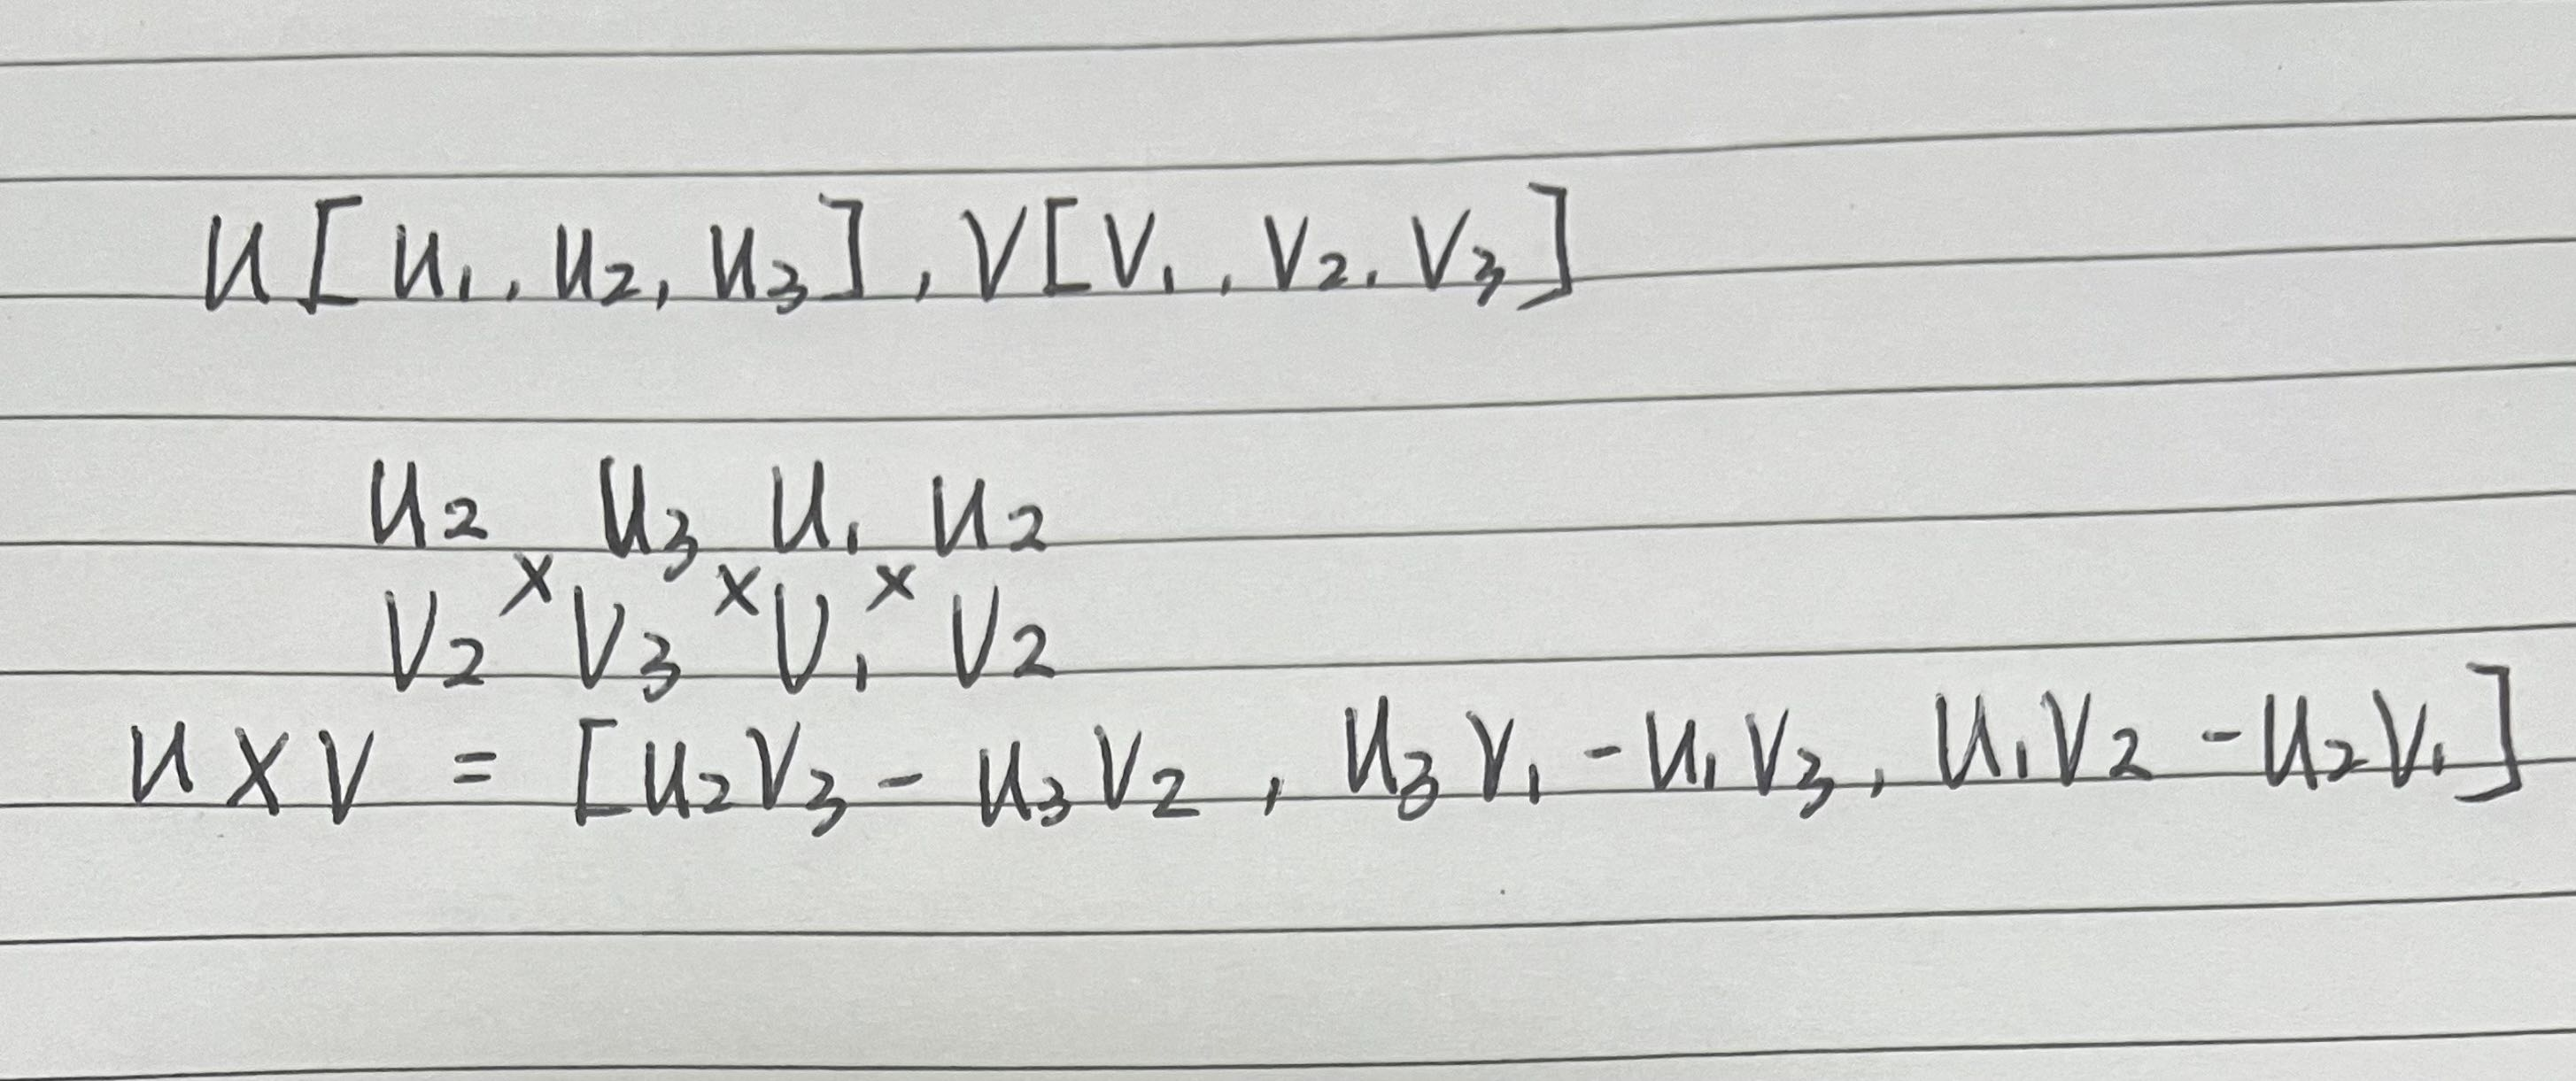
\includegraphics[width=0.9\textwidth]{images/w3-1.jpeg}

\textit{W3-tut-1}

\item  The cross product $\mathbf{u} \times \mathbf{v}$ is orthogonal to both $\mathbf{u}$ and $\mathbf{v}$.

\item  The direction of $\mathbf{u} \times \mathbf{v}$ is given by the right-hand rule.\\

2 - 3 :\\
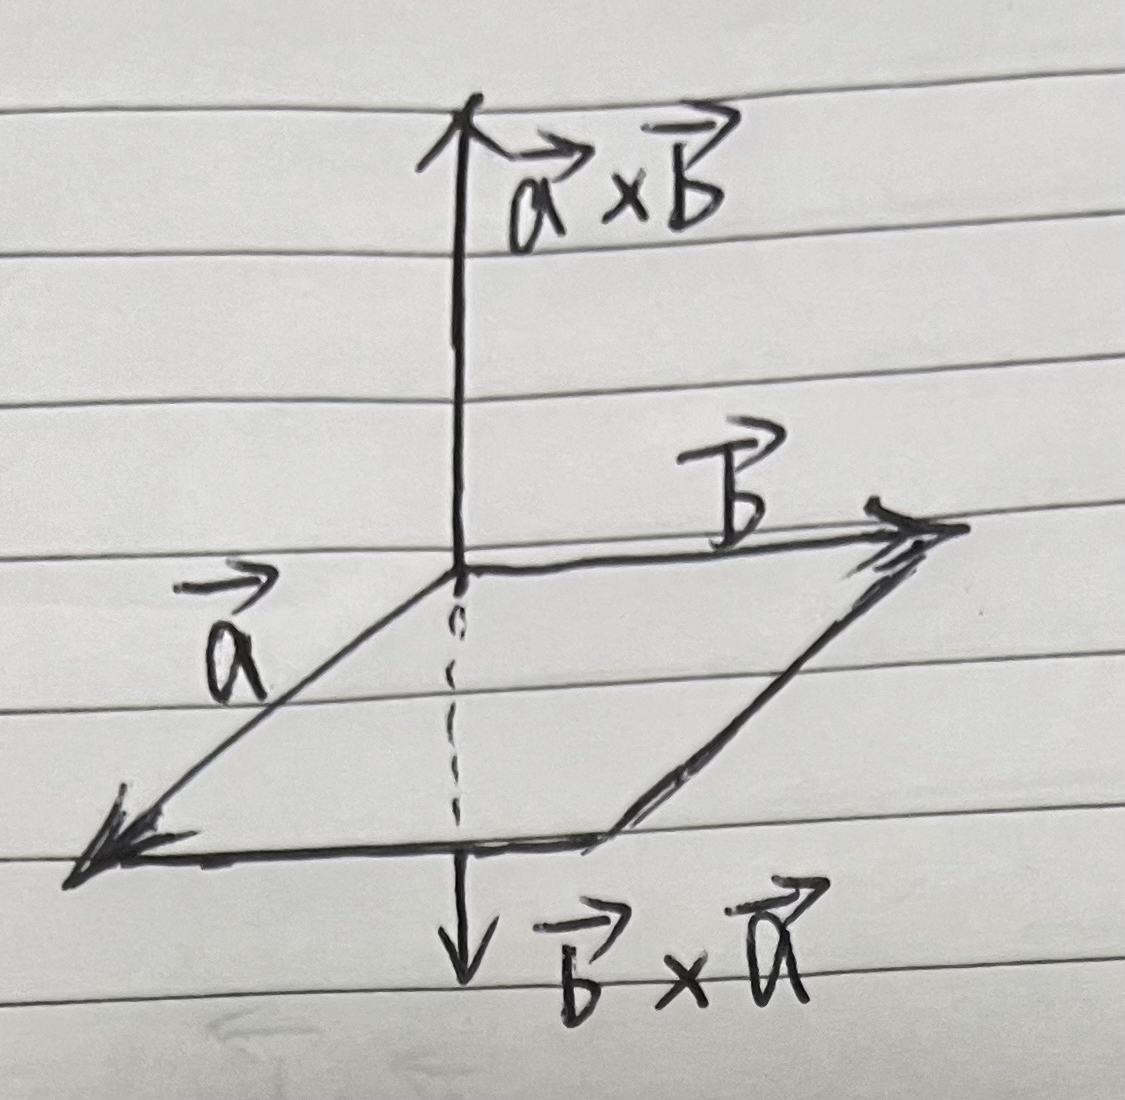
\includegraphics[width=0.5\textwidth]{images/w3-2.jpeg}\\
\textit{W4-tut-4}


\item  \hl{Anti-commutativity of cross product}: For all vectors $\mathbf{u}$ and $\mathbf{v}$ in $\mathbb{R}^{3}, \mathbf{u} \times \mathbf{v}=-(\mathbf{v} \times \mathbf{u})$.

\item  \hl{Distributivity of cross product}: For all vectors $\mathbf{u}, \mathbf{v}$ and $\mathbf{w}$ in $\mathbb{R}^{3}$, $(\mathbf{u}+\mathbf{v}) \times \mathbf{w}=\mathbf{u} \times \mathbf{w}+\mathbf{v} \times \mathbf{w}$

\item  If \hl{$\mathbf{v}$ and $\mathbf{w}$ are vectors in $\mathbb{R}^{3}$ and $c$ is a scalar then : }$(c \mathbf{v}) \times \mathbf{w}=c(\mathbf{v} \times \mathbf{w})=\mathbf{v} \times(c \mathbf{w})$.

\item  For all vectors $\mathbf{u}$ in $\mathbb{R}^{3}, \mathbf{u} \times \mathbf{u}=\mathbf{0}$.

\item  \hl{If $\theta$ is the angle between vectors $\mathbf{v}$ and $\mathbf{w}$ in $\mathbb{R}^{3}$ then}

$$
\|\mathbf{v} \times \mathbf{w}\|=\|\mathbf{v}\|\|\mathbf{w}\| \sin \theta
$$
\\
\textit{W3-tut-4}

\item  \hl{The area of the parallelogram inscribed by $\mathbf{v}$ and $\mathbf{w}$ in $\mathbb{R}^{3}$ is $\|\mathbf{v} \times \mathbf{w}\|$, and the area of the triangle inscribed by $\mathbf{v}$ and $\mathbf{w}$ is $\frac{1}{2}\|\mathbf{v} \times \mathbf{w}\|$.}\\

\textit{assignment1 - 1.1}
\textit{W3-tut-3}

\item  A normal vector for a line $\ell$ is a nonzero vector $\mathbf{n}$ which is orthogonal to any vector parallel to $\ell$.\\
\textit{W4-tut-5}

\item  A direction vector for a line $\ell$ is a nonzero vector $\mathbf{d}$ which is parallel to $\ell$. If $A$ and $B$ are distinct points on $\ell$ then $\overrightarrow{A B}$ is a direction vector for $\ell$

\item  The normal form of the equation for a line $\ell$ in $\mathbb{R}^{2}$ is

$$
\mathbf{n} \cdot(\mathbf{x}-\mathbf{p})=0, \quad \text { or }, \text { equivalently, } \quad \mathbf{n} \cdot \mathbf{x}=\mathbf{n} \cdot \mathbf{p}
$$

where $\mathbf{p}$ is a point on $\ell$, and $\mathbf{n}$ is a normal vector for $\ell$.

\item  The general form of the equation for a line $\ell$ in $\mathbb{R}^{2}$ is

$$
a x+b y=c
$$

where $\mathbf{n}=[a, b]$ is a normal vector for $\ell$.

\item  The vector form of the equation for a line $\ell$ in $\mathbb{R}^{2}$ or $\mathbb{R}^{3}$ is

$$
\mathbf{x}=\mathbf{p}+t \mathbf{d}
$$

where $\mathbf{p}$ is a point on $\ell, \mathbf{d}$ is a direction vector for $\ell$ and $t \in \mathbb{R}$.

$(\mathrm{xv})$ The parametric equations of $\ell$ are the equations corresponding to the components:

$$
x=p_{1}+t d_{1} \quad \text { and } \quad y=p_{2}+t d_{2} \quad\left(\text { and, for lines in } \mathbb{R}^{3}, \quad z=p_{3}+t d_{3}\right), \quad \text { for } t \in \mathbb{R} .
$$

\end{enumerate}





\newpage






\section{Week 4}
\begin{enumerate}
\item The normal form of the equation of a plane $\mathcal{P}$ in $\mathbb{R}^{3}$ is

$$
\mathbf{n} \cdot(\mathbf{x}-\mathbf{p})=0 \quad \text { or equivalently } \quad \mathbf{n} \cdot \mathbf{x}=\mathbf{n} \cdot \mathbf{p}
$$

where $\mathbf{p}$ is a point on $\mathcal{P}$ and $\mathbf{n}$ is a normal vector for $\mathcal{P}$.

\item The general form of the equation for a plane $\mathcal{P}$ in $\mathbb{R}^{3}$ is

$$
a x+b y+c z=d
$$

where $\mathbf{n}=[a, b, c]$ is a normal vector for $\mathcal{P}$.

\item Recall that a vector $\mathbf{v}$ is a linear combination of vectors $\mathbf{v}_{1}, \mathbf{v}_{2}, \ldots, \mathbf{v}_{k}$ if there are scalars $c_{1}, c_{2}, \ldots, c_{k}$ such that

$$
\mathbf{v}=c_{1} \mathbf{v}_{1}+c_{2} \mathbf{v}_{2}+\cdots+c_{k} \mathbf{v}_{k}
$$

The scalars $c_{1}, c_{2}, \ldots, c_{k}$ are the coefficients of this linear combination.

\item \hl{If $S=\left\{\mathbf{v}_{1}, \ldots, \mathbf{v}_{k}\right\}$ is a set of vectors in $\mathbb{R}^{n}$, then the $\operatorname{span}$ of $\mathbf{v}_{1}, \ldots, \mathbf{v}_{k}$, denoted $\operatorname{span}(S)$ or $\operatorname{span}\left(\mathbf{v}_{1}, \ldots, \mathbf{v}_{k}\right)$, is the set of all linear combinations of $\mathbf{v}_{1}, \ldots, \mathbf{v}_{k}$. That is}

$$
\begin{aligned}
\operatorname{span}(S) & =\operatorname{span}\left(\mathbf{v}_{1}, \ldots, \mathbf{v}_{k}\right) \\
& =\left\{\mathbf{v} \in \mathbb{R}^{n}: \mathbf{v}=c_{1} \mathbf{v}_{1}+c_{2} \mathbf{v}_{2}+\cdots+c_{k} \mathbf{v}_{k} \text { for some } c_{1}, c_{2}, \cdots, c_{k} \in \mathbb{R}\right\}
\end{aligned}
$$

\hl{If $\operatorname{span}(S)=\mathbb{R}^{n}$, then $S$ is called a spanning set for $\mathbb{R}^{n}$.}

\item A set of vectors $\mathbf{v}_{1}, \ldots, \mathbf{v}_{k}$ is linearly independent if the only scalars $c_{1}, \ldots, c_{k}$ that satisfy

$$
c_{1} \mathbf{v}_{1}+c_{2} \mathbf{v}_{2}+\cdots+c_{k} \mathbf{v}_{k}=\mathbf{0}
$$

are $c_{1}=c_{2}=\cdots=c_{k}=0$. A set of vectors that is not linearly independent is called linearly dependent.

\item Two non-zero vectors in $\mathbb{R}^{n}$ are linearly independent if and only if they are not parallel.\\
\textit{W4-tut-2}

\item \hl{In $\mathbb{R}^{3}$, the span of any two non-zero non-parallel vectors is the plane through the origin. In other words, let $\mathbf{u}$ and $\mathbf{v}$ be non-zero non-parallel vectors in $\mathbb{R}^{3}$, then the set}

$$
S=\left\{\mathbf{x} \in \mathbb{R}^{3}: \mathbf{x}=s \mathbf{u}+t \mathbf{v}, \text { for some } s, t \in \mathbb{R}\right\}
$$

is the plane through to the origin and parallel to the vectors $\mathbf{u}$ and $\mathbf{v}$.\\
\textit{W4-tut-6}

\item The vector form of the equation for a plane $\mathcal{P}$ in $\mathbb{R}^{3}$ is

$$
\mathbf{x}=\mathbf{p}+s \mathbf{u}+\mathbf{v}
$$

where $\mathbf{p}$ is a point on $\mathcal{P}, \mathbf{u}$ and $\mathbf{v}$ are direction vectors for $\mathcal{P}$ (meaning $\mathbf{u}$ and $\mathbf{v}$ are nonzero and parallel to $\mathcal{P}$, but not parallel to each other), and $s, t \in \mathbb{R}$. The parametric equations of $\mathcal{P}$ are the equations corresponding to the components:

$$
x=p_{1}+s u_{1}+t v_{1}, \quad y=p_{2}+s u_{2}+t v_{2} \quad \text { and } \quad z=p_{3}+s u_{3}+t v_{3} .
$$


\hl{\textit{summarize for vector equations :}} \\\\
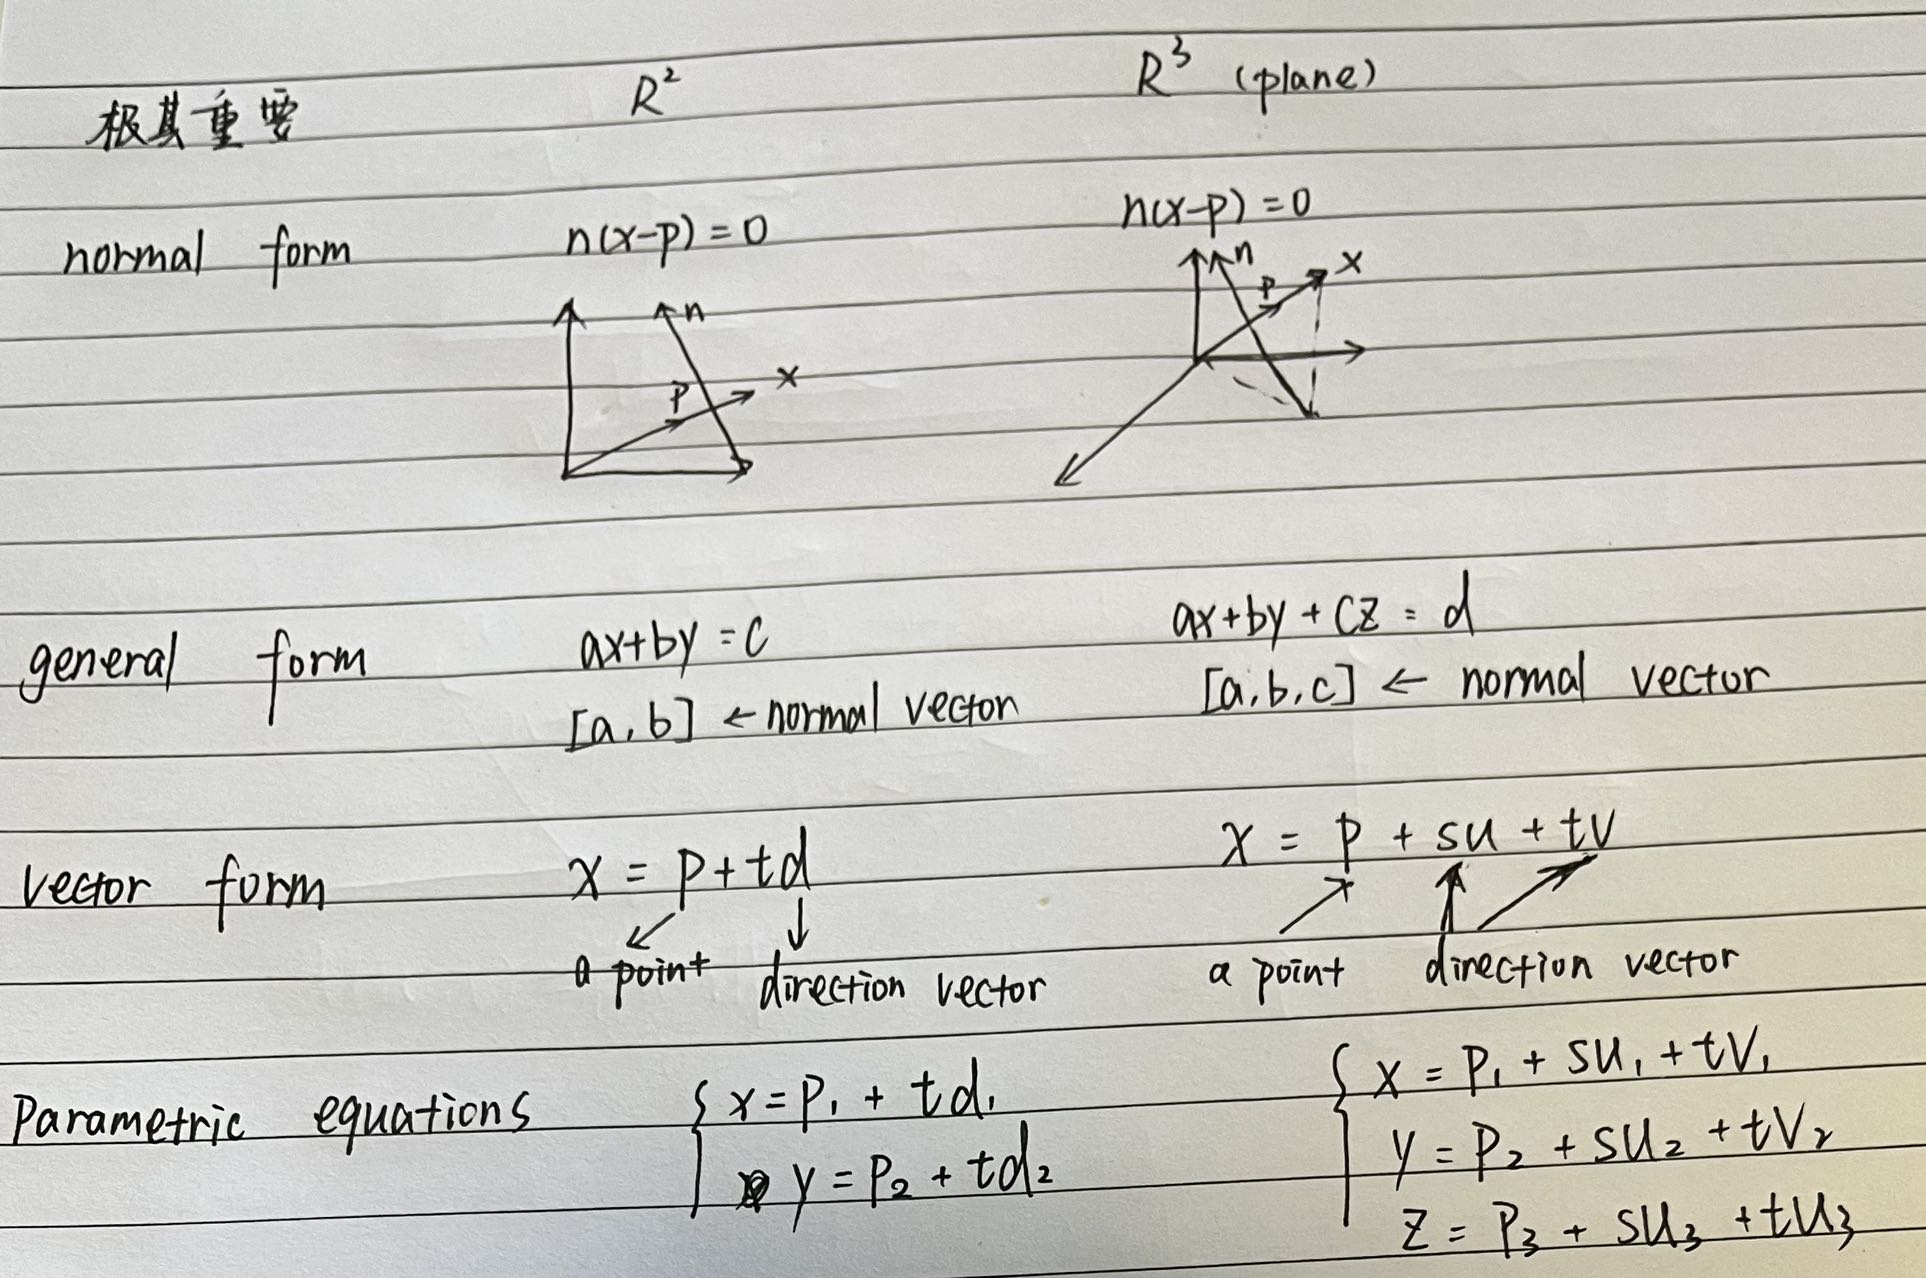
\includegraphics[width=0.9\textwidth]{images/w4-1.jpeg}\\

\textit{W3-tut-5-7}
\textit{W4-tut-1}
\textit{W4-tut-3}
\textit{W4-tut-7-8}

\item If $\mathbf{u}$ and $\mathbf{v}$ are direction vectors for a plane $\mathcal{P}$, then $\mathbf{u} \times \mathbf{v}$ is a normal vector for $\mathcal{P}$.

\item \hl{If $A, B$ and $C$ are three non-collinear points on a plane $\mathcal{P}$, then $\overrightarrow{A B}$ and $\overrightarrow{A C}$ are direction vectors for $\mathcal{P}$, hence $\overrightarrow{A B} \times \overrightarrow{A C}$ is a normal vector to $\mathcal{P}$. }

\item A linear equation in variables $x_{1}, x_{2}, \ldots, x_{n}$ has the form

$$
a_{1} x_{1}+a_{2} x_{2}+\cdots+a_{n} x_{n}=b,
$$

where $a_{1}, a_{2}, \ldots, a_{n}, b$ are constants.

\item A system of linear equations has the form

$$
\begin{aligned}
& a_{11} x_{1}+a_{12} x_{2}+\cdots+a_{1 n} x_{n}=b_{1} \\
& a_{21} x_{1}+a_{22} x_{2}+\cdots+a_{2 n} x_{n}=b_{2} \\
& a_{m 1} x_{1}+a_{m 2} x_{2}+\cdots+a_{m n} x_{n}=b_{m},
\end{aligned}
$$

where the $a_{i j}$ and $b_{i}$, for $1 \leq i \leq m$ and $1 \leq j \leq n$, are constants.

The system is homogeneous if $b_{1}=b_{2}=\cdots=b_{m}=0$.

\item \hl{Every system of linear equations has either no solutions, one solution, or infinitely many solutions. If it has no solutions, then the system is called inconsistent. If it has at least one solution, then the system is called consistent.}

\item The augmented matrix of the system of linear equations in fact (xii) is the matrix

$$
\left[\begin{array}{cccc|c}
a_{11} & a_{12} & \ldots & a_{1 n} & b_{1} \\
a_{21} & a_{22} & \cdots & a_{2 n} & b_{2} \\
\cdots & \cdots & \cdots & \cdots & \cdots \\
a_{m 1} & a_{m 2} & \cdots & a_{m n} & b_{m}
\end{array}\right] .
$$

\item \hl{\textit{appendix : equations for vectors in $\mathbb{R}^{n}$}}\\\\
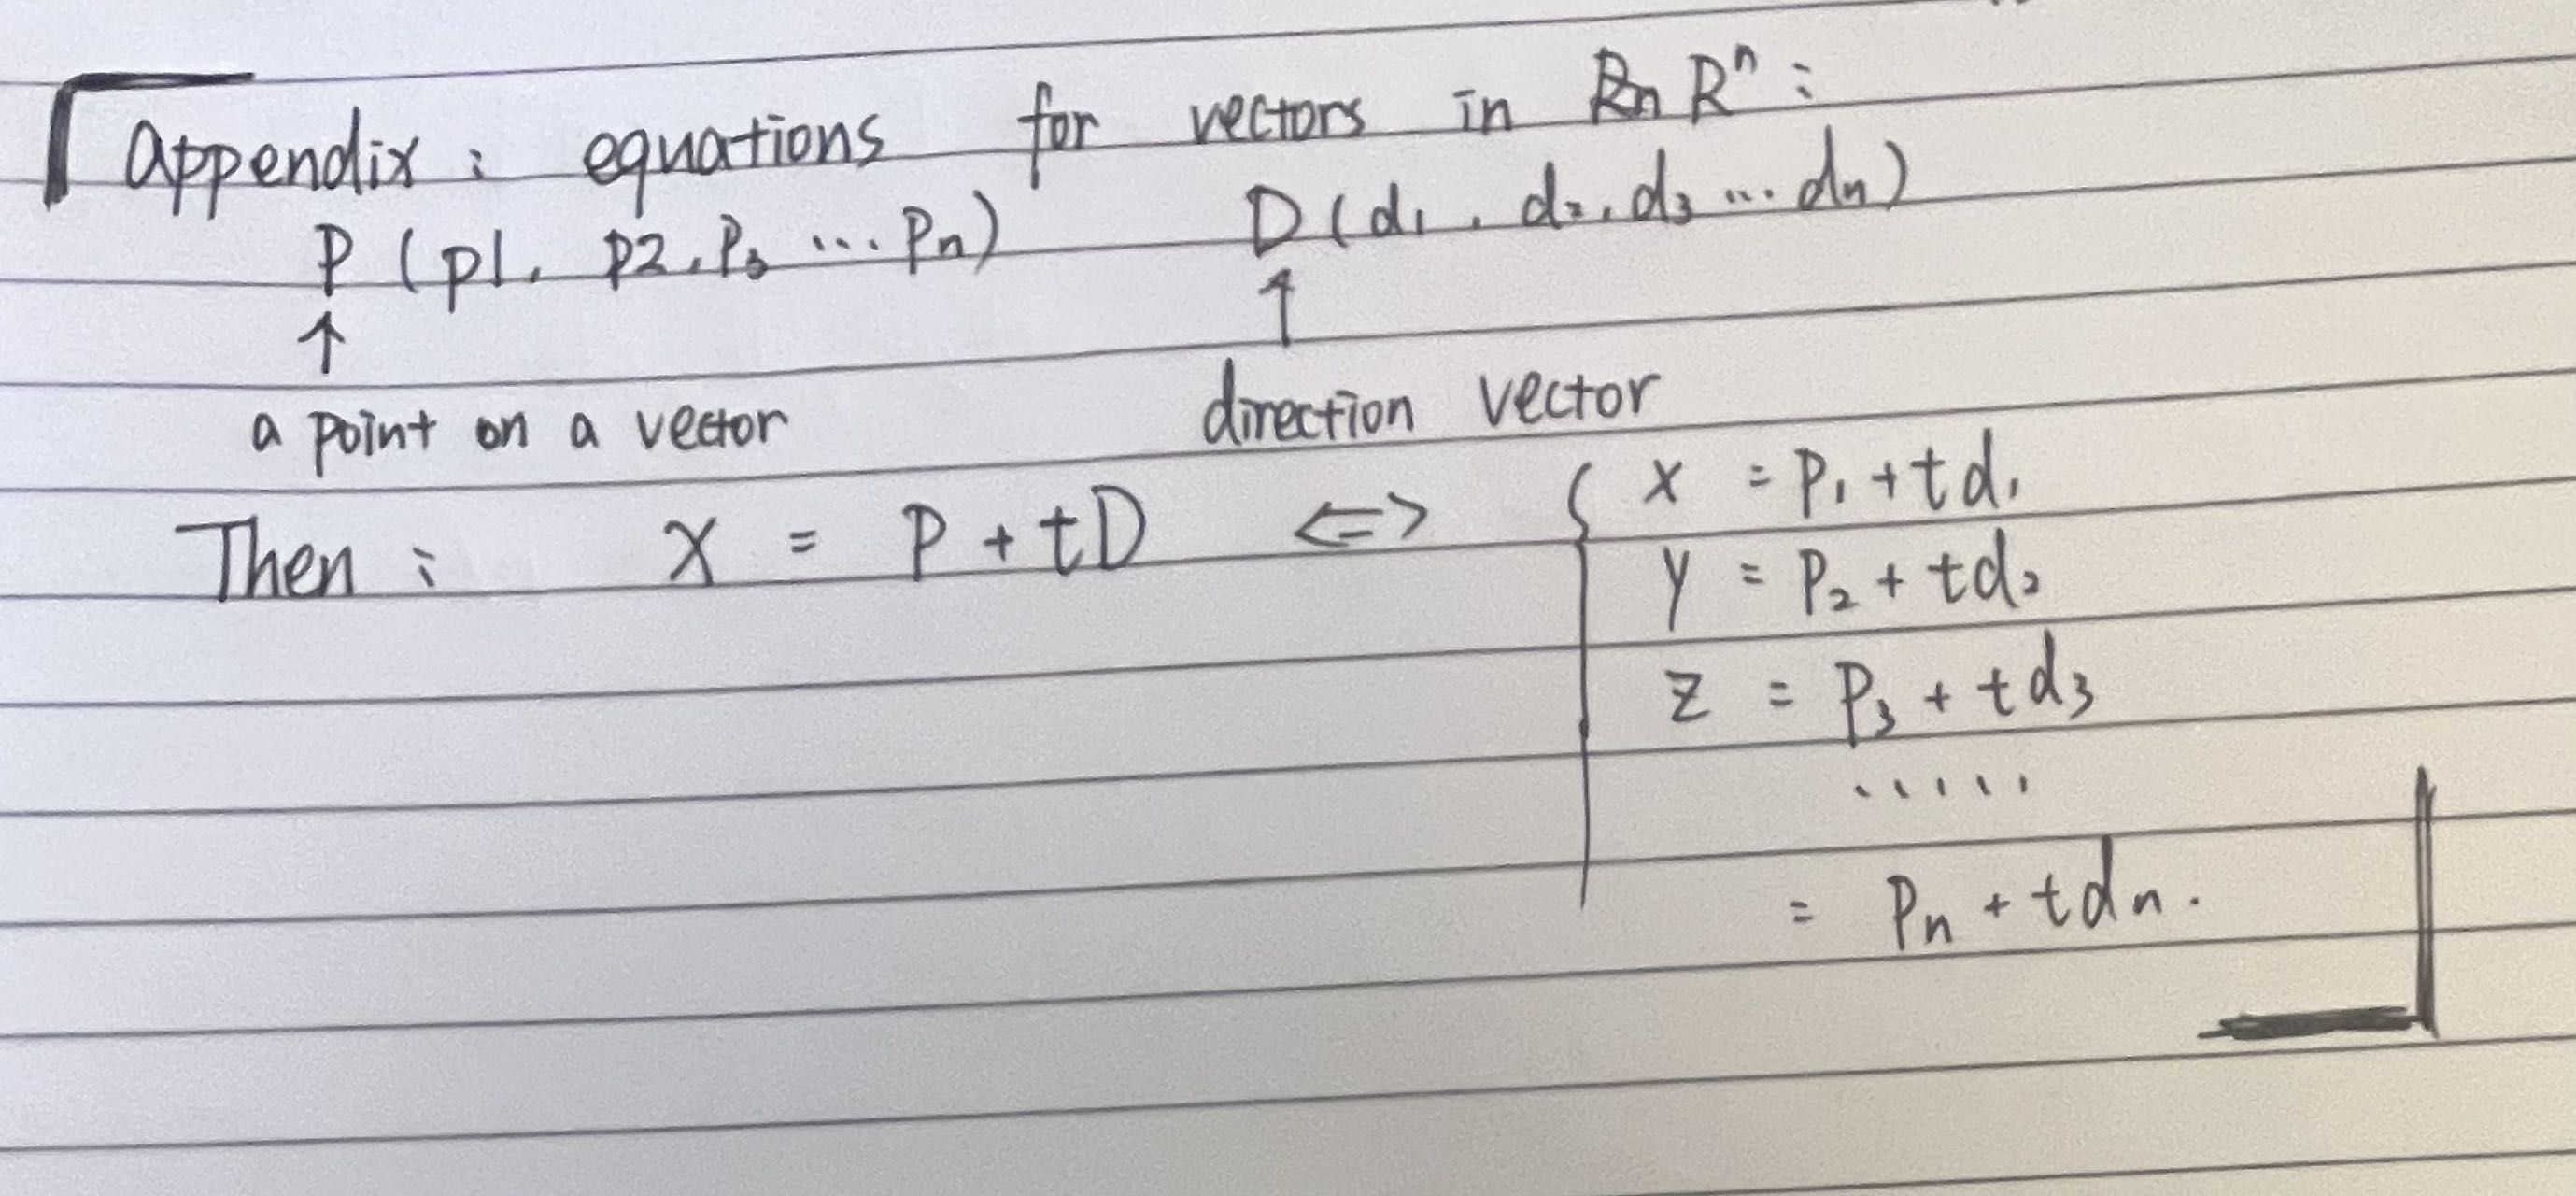
\includegraphics[width=0.9\textwidth]{images/w4-2.jpeg}\\
\textit{assignment1 - 1.2}


\end{enumerate}



\newpage




\section{W5}


\begin{enumerate}


\item A linear equation in variables $x_{1}, x_{2}, \ldots, x_{n}$ has the form

$$
a_{1} x_{1}+a_{2} x_{2}+\cdots+a_{n} x_{n}=b
$$

where $a_{1}, a_{2}, \ldots, a_{n}, b$ are constants.

\item A system of linear equations has the form

$$
\begin{aligned}
& a_{11} x_{1}+a_{12} x_{2}+\cdots+a_{1 n} x_{n}=b_{1} \\
& a_{21} x_{1}+a_{22} x_{2}+\cdots+a_{2 n} x_{n}=b_{2} \\
& a_{m 1} x_{1}+a_{m 2} x_{2}+\cdots+a_{m n} x_{n}=b_{m}
\end{aligned}
$$

where the $a_{i j}$ and $b_{i}$, for $1 \leq i \leq m$ and $1 \leq j \leq n$, are constants.

The system is homogeneous if $b_{1}=b_{2}=\cdots=b_{m}=0$.

\item \hl{Every system of linear equations has either no solutions, one solution, or infinitely many solutions. If it has no solutions, then the system is called inconsistent. If it has at least one solution, then the system is called consistent.}

\item To simplify the solution of a system of linear equations an augmented matrix can be used. It is a matrix

$$
\left[\begin{array}{cccc|c}
a_{11} & a_{12} & \cdots & a_{1 n} & b_{1} \\
a_{21} & a_{22} & \cdots & a_{2 n} & b_{2} \\
\cdots & \cdots & \cdots & \cdots & \cdots \\
a_{m 1} & a_{m 2} & \cdots & a_{m n} & b_{m}
\end{array}\right]
$$

\hl{One can apply the following elementary row operations to the augmented matrix without changing the solutions of the initial system:}

\hl{(a) $R_{i} \leftrightarrow R_{j}($ row swap)}

$$
\left[\begin{array}{cccc|c}
a_{11} & a_{12} & \cdots & a_{1 n} & b_{1} \\
\cdots & \cdots & \cdots & \cdots & \cdots \\
a_{i 1} & a_{i 2} & \cdots & a_{i n} & b_{i} \\
\cdots & \cdots & \cdots & \cdots & \cdots \\
a_{j 1} & a_{j 2} & \cdots & a_{j n} & b_{j} \\
\cdots & \cdots & \cdots & \cdots & \cdots \\
a_{m 1} & a_{m 2} & \cdots & a_{m n} & b_{m}
\end{array}\right] \quad \longrightarrow \quad\left[\begin{array}{cccc|c}
a_{11} & a_{12} & \ldots & a_{1 n} & b_{1} \\
\cdots & \cdots & \cdots & \cdots & \cdots \\
a_{j 1} & a_{j 2} & \cdots & a_{j n} & b_{j} \\
\cdots & \cdots & \cdots & \cdots & \cdots \\
a_{i 1} & a_{i 2} & \cdots & a_{i n} & b_{i} \\
\cdots & \cdots & \cdots & \cdots & \cdots \\
a_{m 1} & a_{m 2} & \cdots & a_{m n} & b_{m}
\end{array}\right]
$$

\hl{(b) $R_{i} \mapsto \lambda R_{i}(\lambda \neq 0$, row scale $)$}

$$
\left[\begin{array}{cccc|c}
a_{11} & a_{12} & \ldots & a_{1 n} & b_{1} \\
\cdots & \cdots & \cdots & \cdots & \cdots \\
a_{i 1} & a_{i 2} & \cdots & a_{i n} & b_{i} \\
\cdots & \cdots & \cdots & \cdots & \cdots \\
a_{m 1} & a_{m 2} & \cdots & a_{m n} & b_{m}
\end{array}\right] \quad \longrightarrow \quad\left[\begin{array}{cccc|c}
a_{11} & a_{12} & \ldots & a_{1 n} & b_{1} \\
\cdots & \cdots & \cdots & \cdots & \cdots \\
\lambda a_{i 1} & \lambda a_{i 2} & \cdots & \lambda a_{i n} & \lambda b_{i} \\
\cdots & \cdots & \cdots & \cdots & \cdots \\
a_{m 1} & a_{m 2} & \cdots & a_{m n} & b_{m}
\end{array}\right]
$$

\hl{(c) $R_{i} \mapsto R_{i}+\lambda R_{j}$ (row add)}

$$
\left[\begin{array}{cccc|c}
a_{11} & a_{12} & \cdots & a_{1 n} & b_{1} \\
\cdots & \cdots & \cdots & \cdots & \cdots \\
a_{i 1} & a_{i 2} & \cdots & a_{i n} & b_{i} \\
\cdots & \cdots & \cdots & \cdots & \cdots \\
a_{j 1} & a_{j 2} & \cdots & a_{j n} & b_{j} \\
\cdots & \cdots & \cdots & \cdots & \cdots \\
a_{m 1} & a_{m 2} & \cdots & a_{m n} & b_{m}
\end{array}\right] \longrightarrow\left[\begin{array}{cccc|c}
a_{11} & a_{12} & \cdots & a_{1 n} & b_{1} \\
\cdots & \cdots & \cdots & \cdots & \cdots \\
a_{i 1}+\lambda a_{j 1} & a_{i 2}+\lambda a_{j 2} & \cdots & a_{i n}+\lambda a_{j n} & b_{i}+\lambda b_{j} \\
\cdots & \cdots & \cdots & \cdots & \cdots \\
a_{j 1} & a_{j 2} & \cdots & a_{j n} & b_{j} \\
\cdots & \cdots & \cdots & \cdots & \cdots \\
a_{m 1} & a_{m 2} & \cdots & a_{m n} & b_{m}
\end{array}\right]
$$

\item \hl{An augmented matrix is in row echelon form if}

\hl{(a) rows of zeroes appear at the bottom}

\hl{(b) the first nonzero entries of consecutive rows appear further to the right}

\hl{(b) Each leading entry is equal to 1}

\item The process of Gaussian elimination applies elementary row operations (row reduction) to transform the augmented matrix of a system into row echelon form, after which the associated system is solved using back substitution:

(a) the leading variables corresponding to leading entries are evaluated one equation at a time from the bottom towards the top,

(b) parameters are assigned to each nonleading variable (if any).

\item \hl{An augmented matrix is in reduced row echelon form if

(a) It is in row echelon form.

(b) The leading entry in each nonzero row is a 1 (called a leading 1 ).

(c) Each column containing a leading 1 has zeros everywhere else.}

\item The process of Gauss-Jordan elimination row reduces the augmented matrix to reduced row echelon form, after which the process of back substitution simplifies. \hl{However, Gauss-Jordan elimination is usually less efficient in terms of the overall number of arithmetic operations used than Gaussian elimination.}


\end{enumerate}


\newpage


\section{W6}

\begin{enumerate}
\item A matrix is an array of numbers, called entries. The plural of matrix is matrices. If a matrix $M$ has $m$ rows and $n$ columns then we say that $M$ is $m \times n$. We call a matrix $M$ square if $M$ is $n \times n$ for some $n$. The entry lying in the $i$ th row and $j$ th column is called the $(i, j)$-entry.

\item A matrix consisting of one row is called a row matrix. A matrix consisting of one column is called a column matrix.

\item \hl{To add or subtract using two matrices of the same size, simply add or subtract the corresponding entries. To form the negative of a matrix, simply take the negatives of its entries.}

\item To multiply a matrix by a scalar, simply multiply all of its entries by the scalar.

\item The zero matrix has all of its entries equal to 0 , and is denoted by 0 , or by $0_{m \times n}$ if it is $m \times n$ and its size needs to be emphasised.

\item \hl{The identity matrix is a square matrix with diagonal entries equal to 1 , and all entries off the diagonal equal to 0. The identity matrix is denoted by $I$, or by $I_{n}$ if it is $n \times n$ and its size needs to be emphasised.}

\item If $A$ is an $m \times n$ matrix and $B$ is an $n \times p$ matrix, then the product $A B$ is defined and is an $m \times p$ matrix. The $(i, j)$-entry of $A B$ is

$$
a_{i 1} b_{1 j}+a_{i 2} b_{2 j}+\cdots+a_{i n} b_{n j}
$$

i.e. the dot product of the $i$ th row of $A$ and the $j$ th column of $B$, for each $1 \leq i \leq m$ and $1 \leq j \leq p$.

\item \hl{The transpose of an $m \times n$ matrix $A$ is the $n \times m$ matrix $A^{T}$ obtained by interchanging the rows and columns of $A$. So the $i$ th column of $A^{T}$ is the $i$ th row of $A$ for all $i$.}

\item \hl{If $A, B$, and $C$ are matrices of the appropriate size (so all of the following sums and products make sense), and $\lambda$ and $\mu$ are scalars, then the following properties hold:}

$$
\begin{gathered}
A+B=B+A, \quad(A+B)+C=A+(B+C), \quad A+0=0+A=A, \\
-(-A)=A, \quad A+(-A)=A-A=0, \quad \lambda(\mu A)=(\lambda \mu) A, \\
\lambda(A+B)=\lambda A+\lambda B, \quad(\lambda+\mu) A=\lambda A+\mu A, \quad I A=A I=A, \\
(A B) C=A(B C), \quad A(B+C)=A B+A C, \quad(A+B) C=A C+B C, \\
\lambda(B C)=(\lambda B) C=B(\lambda C), \quad 0 A=0=A 0 .
\end{gathered}
$$

\item \hl{Warning: Matrix multiplication is not in general commutative. In most cases, we have $A B \neq B A$.}

\item \hl{If $A$ and $B$ are matrices of the appropriate size (so all of the following sums and products make sense), and $\lambda$ and $\mu$ are scalars, then the following properties hold:}

$$
\begin{gathered}
\left(A^{T}\right)^{T}=A, \quad(A+B)^{T}=A^{T}+B^{T}, \quad(\lambda A)^{T}=\lambda\left(A^{T}\right) \\
(A B)^{T}=B^{T} A^{T}, \quad\left(A^{n}\right)^{T}=\left(A^{T}\right)^{n} \quad \text { for all nonnegative integers } n
\end{gathered}
$$
\end{enumerate}




\newpage

\section{W7}
\begin{enumerate}
\item \hl{The inverse of a matrix $A$ is a matrix $A^{-1}$ such that, for some positive integer $n$,}

$$
A A^{-1}=A^{-1} A=I_{n}
$$

\textbf{Only square matrices have inverses.} When it exists, \textbf{the inverse $A^{-1}$ is unique.}

\item \hl{Only half of the definition needs to be checked, in the following sense: if $A$ is a square matrix and $A B=I$ or $B A=I$, then}

$$
A B=B A=I
$$

so that the inverse $A^{-1}$ exists and equals $B$.

\item \hl{Let $A$ be an invertible matrix. Then $A^{T}$ is invertible and $\left(A^{T}\right)^{-1}=\left(A^{-1}\right)^{T}$.}

\item \hl{A matrix is invertible if its inverse exists. If $A$ and $B$ are invertible matrices of the same size, then $A B$ is invertible and $(A B)^{-1}=B^{-1} A^{-1}$.}

\item \hl{For all integers $m, n$ and all nonzero scalars $\lambda$,}

$$
A^{m} A^{n}=A^{m+n}, \quad\left(A^{-1}\right)^{-1}=A, \quad\left(A^{m}\right)^{n}=A^{m n}, \quad(\lambda A)^{-1}=\frac{1}{\lambda} A^{-1}
$$

\item The determinant of a $1 \times 1$ matrix $[a]$ is simply the entry $a$.

\item The determinant of a $2 \times 2$ matrix $A=\left[\begin{array}{ll}a & b \\ c & d\end{array}\right]$ is

$$
\operatorname{det}(A)=\left|\begin{array}{ll}
a & b \\
c & d
\end{array}\right|=a d-b c
$$

\item Let $A=\left[\begin{array}{ll}a & b \\ c & d\end{array}\right]$. \hl{Then $A$ is invertible if and only if $\operatorname{det}(A) \neq 0$, in which case} $A^{-1}=$ $\frac{1}{\operatorname{det}(A)}\left[\begin{array}{rr}d & -b \\ -c & a\end{array}\right]=\frac{1}{a d-b c}\left[\begin{array}{rr}d & -b \\ -c & a\end{array}\right]$

\item \hl{A square matrix $A$ is invertible if and only if the augmented matrix $[A \mid I]$ can be row reduced to $[I \mid B]$, in which case $A^{-1}=B$}

\item \hl{If a system of equations can be expressed in the form $A \mathbf{x}=\mathbf{b}$ where $A$ is invertible, then $\mathbf{x}=A^{-1} \mathbf{b}$.}

\end{enumerate}



\newpage

\begin{enumerate}
\section{W8}
\item \hl{If a system of equations can be expressed in the form $A \mathbf{x}=\mathbf{b}$ where $A$ is invertible, then $\mathbf{x}=A^{-1} \mathbf{b}$.}

\item An \hl{elementary matrix} is any matrix that can be obtained by performing an \hl{elementary row operation on an \textbf{identity matrix}}.

\item \hl{Suppose $E$ is an elementary matrix obtained by performing an elementary row operation on the identity matrix $I_{n}$. If $A$ is an $n \times p$ matrix and we perform the same elementary row operation on $A$, then the resulting matrix is the same as the product $E A$.}

\item The determinant of a $1 \times 1$ matrix $[a]$ is simply the entry $a$.

\item The determinant of a $2 \times 2$ matrix $A=\left[\begin{array}{ll}a & b \\ c & d\end{array}\right]$ is $\operatorname{det}(A)=\left|\begin{array}{ll}a & b \\ c & d\end{array}\right|=a d-b c$.

\item Expanding along any row or down any column of a square matrix $A$ produces the same real number, called the determinant of $A$, denoted by $\operatorname{det}(A)$ (or $\operatorname{det} A$ ) or $|A|$ :

If $A=\left[a_{i, j}\right]$ is an $n \times n$ matrix, then

$$
\operatorname{det}(A)=\sum_{k=1}^{n} a_{i, k} C_{i, k}=\sum_{k=1}^{n} a_{k, j} C_{k, j}
$$

where $C_{i j}=(-1)^{i+j} \operatorname{det} A_{i j}$ is the $(i, j)$-cofactor of $A$, and $A_{i j}$ is the $(i, j)$-minor of $A$, defined as the $(n-1) \times(n-1)$ matrix obtained from $A$ by removing row $i$ and column $j$.

\item The determinant of a $3 \times 3$ matrix $A=\left[\begin{array}{lll}a & b & c \\ d & e & f \\ g & h & k\end{array}\right]$ is

$$
\operatorname{det}(A)=|A|=a\left|\begin{array}{ll}
e & f \\
h & k
\end{array}\right|-b\left|\begin{array}{ll}
d & f \\
g & k
\end{array}\right|+c\left|\begin{array}{ll}
d & e \\
g & h
\end{array}\right|
$$

Note that this is the expansion along the first row (where the smaller determinant arises by ignoring the row and column of the entry being used as a coefficient), but expanding along any row or column is valid, as long as we remember to multiply the determinant of the $(i, j)$-minor of $A$ by $(-1)^{i+j}$. So, for a $3 \times 3$ matrix, we get the following pattern of positive and negative signs:

$$
\left[\begin{array}{lll}
+ & - & + \\
- & + & - \\
+ & - & +
\end{array}\right]
$$

\item If $A$ is triangular, in the sense that all entries above or below the $\operatorname{diagonal}$ are zero, then $\operatorname{det}(A)$ is the product of the diagonal elements.

\item \hl{Determinant method for cross products: If $\mathbf{u}=u_{1} \mathbf{e}_{1}+u_{2} \mathbf{e}_{2}+u_{3} \mathbf{e}_{3}$ and $\mathbf{w}=w_{1} \mathbf{e}_{1}+w_{2} \mathbf{e}_{2}+w_{3} \mathbf{e}_{3}$ then}

$$
\begin{aligned}
\mathbf{u} \times \mathbf{w} & =\left|\begin{array}{ccc}
\mathbf{e}_{1} & \mathbf{e}_{2} & \mathbf{e}_{3} \\
u_{1} & u_{2} & u_{3} \\
w_{1} & w_{2} & w_{3}
\end{array}\right| \\
& =\left(u_{2} w_{3}-u_{3} w_{2}\right) \mathbf{e}_{1}-\left(u_{1} w_{3}-u_{3} w_{1}\right) \mathbf{e}_{2}+\left(u_{1} w_{2}-u_{2} w_{1}\right) \mathbf{e}_{3} \\
& =\left[u_{2} w_{3}-u_{3} w_{2}, u_{3} w_{1}-u_{1} w_{3}, u_{1} w_{2}-u_{2} w_{1}\right]
\end{aligned}
$$

\end{enumerate}



\newpage




\section{W9}
\begin{enumerate}
\item The determinant of a $1 \times 1$ matrix $[a]$ is simply the entry $a$.

\item The determinant of a $2 \times 2$ matrix $A=\left[\begin{array}{ll}a & b \\ c & d\end{array}\right]$ is $\operatorname{det}(A)=\left|\begin{array}{ll}a & b \\ c & d\end{array}\right|=a d-b c$.

\item Expanding along any row or down any column of a square matrix $A$ produces the same real number, called the determinant of $A$, denoted by $\operatorname{det}(A)$ (or $\operatorname{det} A$ ) or $|A|$ :

If $A=\left[a_{i, j}\right]$ is an $n \times n$ matrix, then

$$
\operatorname{det}(A)=\sum_{k=1}^{n} a_{i, k} C_{i, k}=\sum_{k=1}^{n} a_{k, j} C_{k, j}
$$

where $C_{i j}=(-1)^{i+j} \operatorname{det} A_{i j}$ is the $(i, j)$-cofactor of $A$, and $A_{i j}$ is the $(i, j)$-minor of $A$, defined as the $(n-1) \times(n-1)$ matrix obtained from $A$ by removing row $i$ and column $j$.

\item \hl{A quick way to remember the signs is the following "checkerboard" pattern}

$$
\left[\begin{array}{ccccc}
+ & - & + & - & \cdots \\
- & + & - & + & \cdots \\
+ & - & + & - & \cdots \\
- & + & - & + & \cdots \\
\vdots & \vdots & \vdots & \vdots & \ddots
\end{array}\right]
$$

\item \hl{If $A$ is triangular, in the sense that all entries above or below the $\operatorname{diagonal}$ are zero, then $\operatorname{det}(A)$ is the product of the diagonal elements.}

\item \hl{$A$ is invertible if and only if $\operatorname{det}(A) \neq 0$.}

\item \hl{Multiplicative property of the determinant: For any $n \times n$ matrices $A$ and $B$, we have}

$$
\operatorname{det}(A B)=\operatorname{det}(A) \operatorname{det}(B)
$$

\item \hl{If $A$ is invertible then $\operatorname{det}\left(A^{-1}\right)=\frac{1}{\operatorname{det}(A)}$.}

\item \hl{Recall that the transpose $A^{T}$ of a matrix $A$ is the matrix obtained by interchanging rows and columns of $A$. Since the determinant of a matrix can be computed by expanding along any row or column of the matrix, taking the transpose of a matrix does not change its determinant. That is,}

$$
\operatorname{det}\left(A^{T}\right)=\operatorname{det} A
$$

\item \hl{If $B$ is obtained from a matrix $A$ by swapping two rows of $A$ then}

$$
\operatorname{det}(B)=-\operatorname{det}(A)
$$

\item \hl{If $B$ is obtained from a matrix $A$ by adding a scalar multiple of one row of $A$ to another row of $A$, then}

$$
\operatorname{det}(B)=\operatorname{det}(A)
$$

\item \hl{If $B$ is obtained from a matrix $A$ by multiplying a row of $A$ by a scalar $\mu \in \mathbb{R}$, then}

$$
\operatorname{det}(B)=\mu \operatorname{det}(A)
$$

\item \hl{If $A$ is an $n \times n$ matrix, then $\operatorname{det}(k A)=k^{n} \operatorname{det}(A)$.}

\item \hl{Let $A$ be an $n \times n$ matrix. The system $A \mathbf{x}=\mathbf{b}$ has a unique solution if and only if $\operatorname{det}(A) \neq 0$.}

\item Let $A$ be a square matrix, $\mathrm{x}$ a nonzero column vector, and $\lambda$ a scalar such that

$$
A \mathrm{x}=\lambda \mathbf{x}
$$

\hl{Then $\lambda$ is called an eigenvalue of $A$, and $\mathbf{x}$ is called an eigenvector of $A$ corresponding to the eigenvalue $\lambda$. An $n \times n$ matrix has at most $n$ distinct eigenvalues.}

\item A scalar $\lambda$ is an eigenvalue of a square matrix $A$ if and only if

$$
\operatorname{det}(A-\lambda I)=0
$$

\item \hl{The expression $\operatorname{det}(A-\lambda I)$ is a polynomial in $\lambda$ and is called the characteristic polynomial of $A$. The equation $\operatorname{det}(A-\lambda I)=0$ is called the characteristic equation of $A$. The eigenvalues of a matrix are precisely the solutions to its characteristic equation.}

\item \hl{The characteristic polynomial of an $n \times n$ matrix is a degree- $n$ polynomial, and so it has at most $n$ distinct roots. Therefore, an $n \times n$ matrix has \textbf{at most} $n$ distinct eigenvalues.}

\end{enumerate}



\newpage


\section{W10}
\begin{enumerate}
\item Let $A$ be a square matrix, x a nonzero column vector, and $\lambda$ a scalar such that

$$
A \mathbf{x}=\lambda \mathbf{x}
$$

Then $\lambda$ is called an eigenvalue of $A$, and $\mathbf{x}$ is called an eigenvector of $A$ corresponding to the eigenvalue $\lambda$. An $n \times n$ matrix has at most $n$ distinct eigenvalues.

\item A scalar $\lambda$ is an eigenvalue of a square matrix $A$ if and only if

$$
\operatorname{det}(A-\lambda I)=0
$$

\item The expression $\operatorname{det}(A-\lambda I)$ is a polynomial in $\lambda$ and is called the characteristic polynomial of $A$. The equation $\operatorname{det}(A-\lambda I)=0$ is called the characteristic equation of $A$. The eigenvalues of a matrix are precisely the solutions to its characteristic equation.

\item The characteristic polynomial of an $n \times n$ matrix is a degree- $n$ polynomial, and so it has at most $n$ distinct roots. Therefore, an $n \times n$ matrix has at most $n$ distinct eigenvalues.

\item Finding the eigenspace corresponding to the eigenvalue $\lambda$ of a matrix $A$ is equivalent to solving the homogeneous system with coefficient matrix $A-\lambda I$. After the eigenspace has been found, substituting in particular nonzero values of the parameters yields particular eigenvectors.

\item If $A$ is a triangular matrix, in the sense that all of the entries above or below the diagonal are zero, \hl{then $\operatorname{det}(A)$ is equal to the product of all of the diagonal entries of $A$. }\textbf{This implies that the eigenvalues of a triangular matrix are simply the diagonal entries of the matrix.}

\item The algebraic multiplicity of an eigenvalue of a matrix is its multiplicity as a root of the characteristic equation. So, for instance, if the characteristic equation is $(\lambda-2)(\lambda-5)^{4}=0$, then the algebraic multiplicity of $\lambda=2$ is 1 , and the algebraic multiplicity of $\lambda=5$ is 4 .

\item The geometric multiplicity of an eigenvalue $\lambda$ of the matrix $A$ is the number of free variables in the set of solutions of $(A-\lambda I) \mathbf{x}=\mathbf{0}$ (or equivalently the number of columns without leading entries in the row echelon form of the augmented matrix $[A-\lambda I \mid \mathbf{0}])$.

\item The geometric multiplicity of each eigenvalue of a square matrix is less than or equal to its algebraic multiplicity.

\item Let $A=\left[a_{i j}\right]$ be an $n \times n$ matrix. The trace of $A$ is defined by

$$
\operatorname{tr}(A)=a_{11}+a_{22}+\cdots a_{n n}=\sum_{i=1}^{n} a_{i i} .
$$

In other words, the trace of $A$ is the sum of all elements on the main diagonal.

\item Let $\lambda_{1}, \lambda_{2}, \ldots, \lambda_{n}$ be a complete set of eigenvalues (repetition included) of the $n \times n$ matrix $A$, then

$$
\operatorname{tr}(A)=\lambda_{1}+\lambda_{2}+\cdots+\lambda_{n}, \quad \text { and } \quad \operatorname{det}(A)=\lambda_{1} \lambda_{2} \cdots \lambda_{n} .
$$






\end{enumerate}


\newpage

\section{W11}

\begin{enumerate}
\item A square matrix $D$ is diagonal if all entries off the diagonal are zero.

\item If $D$ and $E$ are diagonal matrices, then $D E$ is also diagonal, and its diagonal entries are simply the products of corresponding diagonal entries of $D$ and $E$.

\item For all integers $n \geq 0$, the diagonal entries of $D^{n}$ are just the $n$th powers of the diagonal entries of $D$. If $D$ is invertible, then the diagonal entries of $D^{-n}$ are the $(-n)$ th powers of the diagonal entries of $D$.

\item A matrix $A$ is diagonalisable if there is an invertible matrix $P$ and a diagonal matrix $D$ such that

$$
A=P D P^{-1}
$$

\hl{In other words, a matrix $A$ is diagonalisable if there is an invertible matrix $P$ such that the matrix $P^{-1} A P$ is diagonal.}

\item Let $A$ be an $n \times n$ matrix with eigenvalues $\lambda_{1}, \ldots, \lambda_{n}$, and corresponding eigenvectors $\mathbf{v}_{1}, \ldots, \mathbf{v}_{n}$. Then

$$
A P=P D
$$

where $D$ is the diagonal matrix with eigenvalues of $A$ down the diagonal, and $P$ is the matrix with corresponding eigenvectors as columns (i.e. in the columns corresponding to the positions of the corresponding eigenvalues in $D$ ). If $P$ is invertible, then

$$
A=P D P^{-1} \text { and } D=P^{-1} A P
$$

for all integers $n \geq 0$

\item In fact $(\mathrm{v})$, if the eigenvalues of $A$ are all distinct, then $P$ is invertible, and $A$ is diagonalisable. (Note that it is possible for an $n \times n$ matrix to be diagonalisable even if it doesn't have $n$ distinct eigenvalues.)

\item \textbf{The Diagonalisation Theorem}: An $n \times n$ matrix $A$ is diagonalisable if and only if it has $n$ linearly \hl{independent eigenvectors}. \textbf{Also}, an $n \times n$ matrix $A$ is diagonalisable if and only if the \hl{algebraic multiplicity} of each eigenvalue is equal to its \hl{geometric multiplicity}.

\item If $A$ is diagonalisable, then powers of $A$ can be found efficiently using the formula

$$
A^{n}=P D^{n} P^{-1}
$$

for $n \in \mathbb{Z}$ and $n \geq 0$

\item In general, if $A$ and $B$ are $n \times n$ matrices, and there exists an invertible $n \times n$ matrix $P$ such that $A=P B P^{-1}$, then we say that $A$ is similar to $B$, and we write $A \sim B$. (Note that we don't need $A$ or $B$ to be diagonal in order for $A$ to be similar to $B$.)

\item Leslie model of population growth.

\begin{itemize}
  \item The population is divided into $k$ age groups of equal duration.

  \item For each age group $0 \leq i \leq k$, we are given the birth parameter $b_{i}$ equal to the average number of females produced by a female in the age group $i$ (so $\left.b_{i} \geq 0\right)$.

  \item For each age group $0 \leq i \leq k-1$, we are given the survival probability $s_{i}$ equal to the probability that a female in age group $i$ survives into age group $i+1\left(\right.$ so $\left.0 \leq s_{i} \leq 1\right)$. - The Leslie matrix for the model is

\end{itemize}

$$
L=\left[\begin{array}{cccccc}
b_{1} & b_{2} & b_{3} & \cdots & b_{k-1} & b_{k} \\
s_{1} & 0 & 0 & \cdots & 0 & 0 \\
0 & s_{2} & 0 & \cdots & 0 & 0 \\
0 & 0 & s_{3} & \cdots & 0 & 0 \\
\vdots & \vdots & \vdots & \ddots & \vdots & \vdots \\
0 & 0 & 0 & \cdots & s_{k-1} & 0
\end{array}\right]
$$

\begin{itemize}
  \item If $\mathbf{x}_{\mathbf{n}}$ is the distribution of the female population among the age groups after $n$ time periods (so $\mathbf{x}_{\mathbf{0}}$ is the initial distribution of female population), then
\end{itemize}

$$
\mathbf{x}_{\mathbf{n}}=L^{n} \mathbf{x}_{\mathbf{0}}
$$

(\textbf{Note}: This is only an approximation, since the right-hand side might be a vector with noninteger entries, while $\mathbf{x}_{\mathbf{n}}$ always only has integer entries.)
\end{enumerate}


\newpage


\section{W12}
\begin{enumerate}
  \item A probability vector is a vector $\mathbf{y}=\left[y_{1}, \ldots, y_{k}\right]$ such that $0 \leq y_{i} \leq 1$ for all $1 \leq i \leq k$, and $\sum_{i=1}^{k} y_{i}=1$

  \item We call a matrix $P$ a stochastic matrix if each column of $P$ is a probability vector. (So all entries of a stochastic matrix are nonnegative, and the entries in each column sum to 1).

  \item We say that a stochastic matrix $P$ is regular if there exists an integer $m>0$ such that all entries of the matrix $P^{m}$ are positive.

  \item A stochastic process is a collection of random variables representing the random evolution of some system over time.

  \item A stochastic process with $k$ states is called a Markov chain if the transition probabilities from the state $j$ to the state $i$ are time-independent. We denote the probability of transitioning from state $j$ to state $i$ by $p_{i j}$

\begin{itemize}
  \item For every $1 \leq i, j \leq k$, we have $0 \leq p_{i j} \leq 1$

  \item For every $1 \leq j \leq k$, we have $\sum_{i=1}^{k} p_{i j}=1$.

  \item The transition matrix of the Markov chain is the $k \times k$ matrix $P=\left(p_{i j}\right)$. (Note that $P$ is a stochastic matrix.)

  \item We denote by $\mathbf{x}_{n}$ the population distribution at time $n$, and call it a state vector. The initial population distribution (at time zero) is $\mathbf{x}_{0}$. We have

\end{itemize}

$$
\mathbf{x}_{n}=P^{n} \mathbf{x}_{0}, \text { for all integers } n \geq 0
$$

\begin{itemize}
  \item The probability of transitioning from state $j$ to state $i$ in $n$ steps is equal to the $(i, j)$-entry of the matrix $P^{n}$

  \item We say that a Markov chain is regular if its transition matrix $P$ is regular (\hl{that is, if there exists a time $m$ such that the probability of transitioning from any initial state $j$ to any state $i$ in $m$ steps is positive}).

  \item If the transition matrix $P$ is regular, then for every initial probability distribution $\mathbf{x}_{0}$, we have $x_{n}=P^{n} \mathbf{x}_{0} \rightarrow \mathbf{x}$, where $\mathbf{x}$ is the \hl{steady-state vector satisfying $P \mathbf{x}=\mathbf{x}$,} with nonnegative entries that sum to the total population (which is the sum of the entries of $\mathbf{x}_{0}$ ). This is referred to as the asymptotic behaviour (or long-term behaviour) of the Markov chain.

  \item The steady-state probability vector is the unique vector $\mathbf{x}$ satisfying $P \mathbf{x}=\mathbf{x}$, with nonnegative entries that sum to 1 .

  \item Let $P$ be a regular transition matrix of a Markov chain. Then as $k \rightarrow \infty$, the matrix $P^{k}$ approaches the matrix $L=\left[\begin{array}{lll}\mathbf{x} \mathbf{x} & \cdots  \mathbf{x}\end{array}\right]$, where $\mathbf{x}$ is the \textbf{steady-state probability vector} (i.e. $P \mathbf{x}=\mathbf{x}$, the entries of $\mathbf{x}$ are all nonnegative, and the sum of the entries of $\mathbf{x}$ is 1$)$. We call $L$ the long-range transition matrix of the Markov chain.

\end{itemize}

  \item \hl{If $P$ is the transition matrix of a Markov chain, then $\lambda=1$ is an eigenvalue of $P$.}

  \item Let $P$ be a transition matrix of a Markov chain with eigenvalue $\lambda$. Then $|\lambda| \leq 1$. If $P$ is regular and $\lambda \neq 1$, then $|\lambda|<1$. (That is, if $P$ is regular, then -1 is not an eigenvalue of $P$.)


\end{enumerate}



\end{document}